\documentclass[12pt,notitlepage,oneside]{report}

\usepackage{buetcseugthesis}

% Uncomment the following line if you need to write in Bangla
% \usepackage{usebangla}

% Uncomment any of the following lines should you need to
% suppress the LOF, or LOT or LOA

% \suppresslistoffigures 
% \suppresslistoftables
% \suppresslistofalgorithms

% For index creation, comment this out if you do not want to create an
% index
\makeindex[intoc]

\begin{document}

% Edit as needed below this line
% %%%%%%%%%%%%%%%%%%%%%%%%%%%%%%%%%%%%%%%%%%%%%%%%%%%%%%%%

% Chapter-1 Introduction
\chapter{Introduction}\label{intro}

Map digitization is the process of constructing vector based shapes from scanned paper maps. There has been some major research on the extraction of features from raster maps to vector format. Traditional mouza maps have a limited size. Therefore representing them in digital format provides with additional scopes and features. When these maps are digitized, their manipulation, property extraction an representation becomes straightforward. 

The main hurdles with vectorizing the map is to find the actual plotlines that require vectorization. Traditional image scan leaves several noise factors that reduce accuracy of feature extraction. These include but are not limited to: paper crease, ink smear, missing ink, overlap, smear etc. Extracting the actual contours of the plots by removing noise and linking missing links is the objective of this thesis.

This chapter will introduce the topics and briefly discuss about motivation behind this thesis, summary of existing works, limitations and objectives.

\section{Problem Statement and Motivation}

The problem statement is \textbf{\textit{``Mouza Land Map Digitization''}}. Here digitization refers to feature extraction of morphological mouza maps to vectorize the plot contours and assign necessary data to the plots.

The proposed automated method will eliminate noise and perform edge linking, contour and number extraction and reconstruction of the plot from vector subsegments.

There is currently no system in place to make the whole process automated from scanned image to noise reduction to number and contour recognition and georeferencing feature extraction. Raster to vector is necessary for the overlay feature and to provide sufficient accuracy at different zoom level.

The motivation behind this thesis is to automate the whole process of digitizing the mouza maps in such a way that:
\begin{enumerate}
\item Mouza plot information can be easily accessible and representable.
\item The information can be overlaid on any complex background such as topographical, topological, land cover, land use maps or even google map due to georeferencing.
\item Final digitized output can be modified with GIS and automatically reconstruct complex maps through divide and conquer.
\item preservation data accuracy.
\end{enumerate}

\section{Summary of Existing Works and Limitations}

Several ideas of morphological map segmentation have been proposed so far. 
In~\cite{Panja003} the author deals with the problem based on assumptions that most of the extracted features will be of regular polygon. In~\cite{632031} authors have used the underlying property of lines to extract structural information. In~\cite{6065540} authors have focused on determining the text of a map with varying orientation and size. In~\cite{206957,YAMADA1991479} authors have proposed an approach that detects layers in a map in parallel. Besides these other map extraction processes have also been introduced. This literature review will be discussed elaborately in chapter 3. 

The main limitation of the existing work is that there is no complete automated process of map feature extraction curtailed to the specific set of requirements in mouza map digitization. The approaches all refer to different subproblems but are not automated to the last required output. Some have problem domain very dissimilar to that of the mouza maps, like~\cite(4512313) deals specifically with assigning altitude value to scanned contour maps.

\section{Objectives}

The main objectives of this thesis is to automate the following aspects of feature extraction and utilisation:
\begin{enumerate}
\item Compensating and correcting the inherent limitations of a scanned paper map.
\item Georeferencing the extracted plot informations
\item Progressive reconstruction of parent map from multiple submaps.
\end{enumerate}

\section{Scope of the Thesis}

The domain of this problem is not limited to the scope of this thesis. The following aspects are not in the purview of this work:
\begin{enumerate}
\item Recognising and interpreting the various texts and symbols present in standard Mouza maps.
\item Georeferencing with Latitude/Longitude, UTM or GPS data.
\item Joining different Mouza maps
\end{enumerate}

\section{Organization of the Thesis}

We have divided our work plan in several chapters. Chapter \ref{intro} is introduction which contains our topics and brief discussion about motivation behind the topics, summary of existing works, limitations and objectives. Chapter \ref{ch:term} includes some terminologies regarding our thesis. Chapter \ref{ch:review} contains the publications consulted in this thesis. Chapter \ref{ch:workplan} proposes the guidelines for this work.



\endinput


% Terminologies
\chapter{Background}\label{ch:term}

\section{Introduction}

Image processing is a method to perform some operations on an image, in order to get an enhanced image or to extract some useful information from it. It is a type of signal processing in which input is an image and output may be image or characteristics/features associated with that image~\cite{dip}. In this work we deal with a broad spectrum of image processing techniques.

Morphological image analysis is the subsection of Digital Image Processing that we are most interested in. Binary images may contain numerous imperfections. In particular, the binary regions produced by simple thresholding are distorted by noise and texture. Morphological image processing pursues the goals of removing these imperfections by accounting for the form and structure of the image. These techniques can be extended to greyscale images.

Morphological image processing is a collection of non-linear operations related to the shape or morphology of features in an image. morphological operations rely only on the relative ordering of pixel values, not on their numerical values, and therefore are especially suited to the processing of binary images. Morphological operations can also be applied to greyscale images such that their light transfer functions are unknown and therefore their absolute pixel values are of no or minor interest. 

Most of the terms needed for this thesis are related to morphological image processing.In this chapter we will discuss some terminologies regarding this thesis.

\section{Preliminaries}

\subsection{RGB Color to Grayscale Image Conversion}
An RGB image is a three $M*N$ size color components image where the components are red(R), green(G) and blue(B). Color intensity of each component is represented by an 8 bit number. Figure 2.1 shows an RGB color image.

Grayscale image ~\cite{vincent1993morphological} is simply black and white image where it is represented by only one intensity components. It has infinite colors where the brightest color is white and darkest color is black. The color intensity of grayscale image is represented by 8 bit number where the value 0 means white and 255 means black. Figure 2.2 shows the grayscale image. An RGB color image can be converted to Grayscale image using different weighting of red, green and blue color components. The equation can be following 

\begin{equation}
Gray(i,j)=0.40*R(i,j)+ 0.60*G(i,j)+0.30*B(i,j)
\end{equation}

``\Cref{fig:RGB to GrayScale Image} shows RGB to GrayScale Image conversion''.

\vspace{50pt}
\begin{figure}[H]
  \centering
  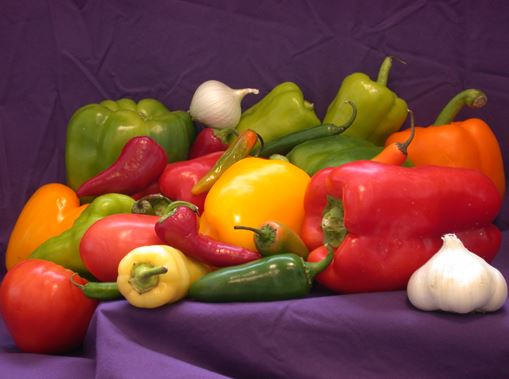
\includegraphics[height=0.6\textwidth,,keepaspectratio]{figures/2_2_1a}
  \caption{RGB Image}
  \label{fig:RGB Image Example}
\end{figure}

\vspace{40pt}
\begin{figure}[H]
  \centering
  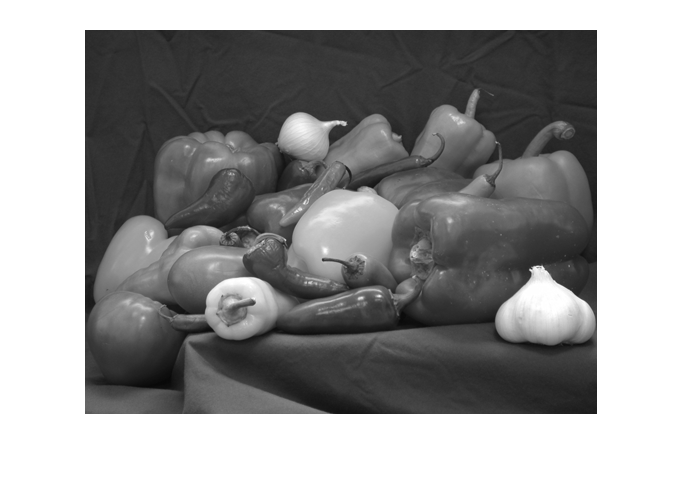
\includegraphics[width=0.9\textwidth]{figures/2_2_1b}
  \caption{Gray Scale Image}
  \label{fig:RGB to GrayScale Image}
\end{figure}

\subsection{Grayscale to Binary Image Conversion}
Binary images ~\cite{russ1995image} are the special kind of image whose intensity value has only two possible values. The image consists of two colors black and white and they are numerically represented by 0 and 1. The intensity value 0 means black and 1 means white. ``\Cref{fig:Grayscale to Binary Image Conversion} shows Grayscale to Binary Image conversion''.
\\

\begin{figure}[h]
  \centering
  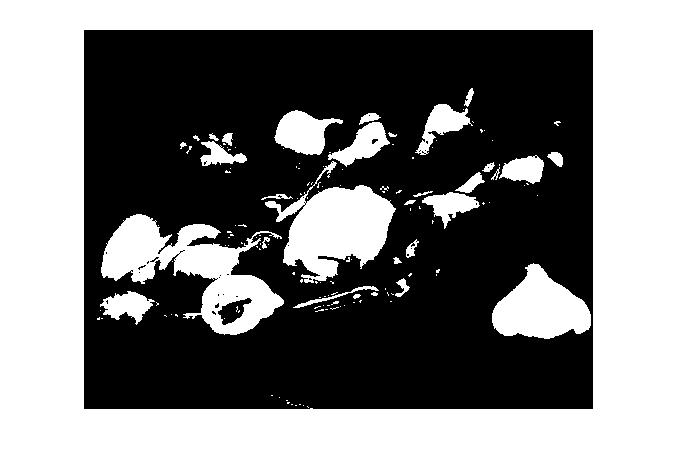
\includegraphics[width=0.9\textwidth]{figures/2_2_2}
  \caption{Grayscale to Binary Image Conversion}
  \label{fig:Grayscale to Binary Image Conversion}
\end{figure}

Basically, binary images are produced by thresholding a grayscale image or a  RGB  using a threshold intensity value and the objective of binarization is to separate the object from the background  image. Usually object color is white and referred to as the foreground color and the rest color is referred as the background color which is black. 

\section{Mask Image}

In image processing, a kernel, convolution matrix, or mask is a small matrix. It is used for blurring, sharpening, embossing, edge detection, image substraction, addition and more. This is accomplished by doing a convolution between a kernel and an image.  Masking involves setting some of the pixel values in an image to zero, or some other "background" value. A mask image is simply an image where some of the pixel intensity values are zero, and others are non-zero.


\subsection{Gaussian Filter}
Image blurring is achieved by convolving the image with a low-pass filter kernel. It is useful for removing noise. It
actually removes high frequency content (e.g: noise, edges) from the image resulting in edges being blurred when this
is filter is applied.

Probably the most useful filter (although not the fastest). Gaussian filtering is done by convolving each point in the input array with a Gaussian kernel and then summing them all to produce the output array. ``\Cref{fig:Gaussian} shows Gaussian Filtering''.

\begin{equation}
G(x,y) = \frac{1}{2 \pi \sigma ^{2}} e^{- \frac{x^{2} + y^{2}}{2 \sigma ^{2}}}
\label{2dgaussian}
\end{equation}

\vspace{50pt}
\begin{figure}[H]
  \centering
  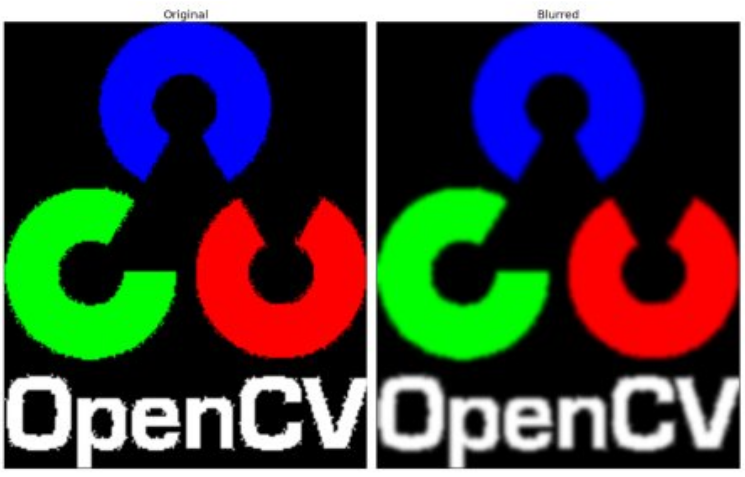
\includegraphics[width=0.9\textwidth]{figures/Gaussian}
  \caption{Gaussian Blur}
  \label{fig:Gaussian}
\end{figure}

\subsection{Median Filter}

The median filter run through each element of the signal (in this case the image) and replace each pixel with the median of its neighboring pixels (located in a square neighborhood around the evaluated pixel). ``\Cref{fig:Median} shows Median Filtering''.

\vspace{50pt}
\begin{figure}[H]
  \centering
  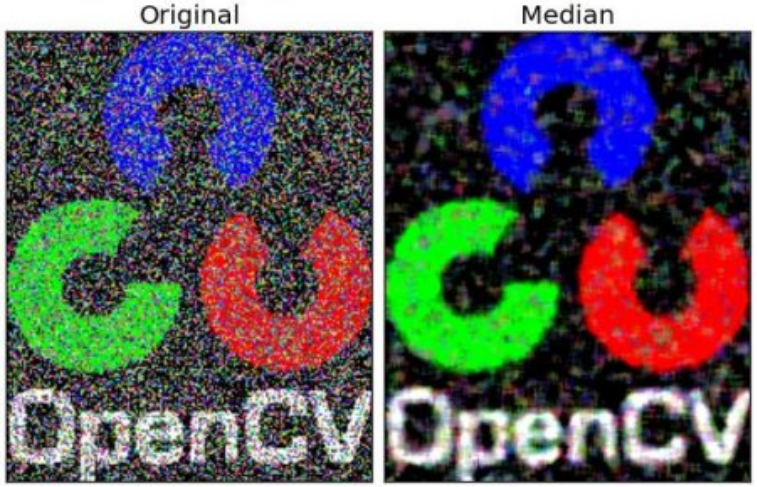
\includegraphics[height=0.4\textwidth,,keepaspectratio]{figures/Median}
  \caption{Median}
  \label{fig:Median}
\end{figure}

\section{Fundamental Operations in Morphological Image Processing}

Some of the more common operations of Morphological Image Processing are mentioned below:

\subsection{Erosion and Dilation}

The basic idea of erosion is just like soil erosion only, it erodes away the boundaries of foreground object (Always
try to keep foreground in white). So what does it do? The kernel slides through the image (as in 2D convolution). A
pixel in the original image (either 1 or 0) will be considered 1 only if all the pixels under the kernel is 1, otherwise it
is eroded (made to zero).

So what happens is that, all the pixels near boundary will be discarded depending upon the size of kernel. So the
thickness or size of the foreground object decreases or simply white region decreases in the image. It is useful for
removing small white noises (as we have seen in colorspace chapter), detach two connected objects etc.

Dilation is just the opposite of erosion. So it increases the white region in the image or size of foreground object increases. Normally, in cases like noise removal, erosion is followed by dilation. Because, erosion removes white noises, but it also shrinks our object. So we dilate it. Since noise is gone, they won’t come back, but our object area increases. It is also useful in joining broken parts of an object.

\begin{figure}[htp]

\centering

\includegraphics[width=.3\textwidth]{figures/Original}\hfill

\includegraphics[width=.3\textwidth]{figures/Erosion}\hfill

\includegraphics[width=.3\textwidth]{figures/Dilation}

\caption{From Left: Original Image, Eroded Image, Dilated Image}
\label{fig:Morpho}

\end{figure}


\subsection{Morphological Opening and Closing}
Opening is just another name of erosion followed by dilation. It is useful in removing noise, as explained above. ``\Cref{fig:Opening} shows Morphological Opening''.

Closing is reverse of Opening, Dilation followed by Erosion. It is useful in closing small holes inside the foreground
objects, or small black points on the object. ``\Cref{fig:Closing} shows Morphological Closing''.

\vspace{50pt}
\begin{figure}[H]
  \centering
  
\includegraphics[height=0.4\textwidth,,keepaspectratio]{figures/Opening}
  \caption{Morphological Opening}
  \label{fig:Opening}
\end{figure}

\vspace{50pt}
\begin{figure}[H]
  \centering
  
\includegraphics[height=0.4\textwidth,,keepaspectratio]{figures/Closing}
  \caption{Morphological Closing}
  \label{fig:Closing}
\end{figure}

\section{Image Segmentation}

In image processing, image segmentation is the process of partitioning a digital image into multiple segments (sets of pixels, also known as super-pixels). The goal of segmentation is to simplify and/or change the representation of an image into something that is more meaningful and easier to analyze.~\cite{shapiro2001computer} Image segmentation is typically used to locate objects and boundaries (lines, curves, etc.) in images. More precisely, image segmentation is the process of assigning a label to every pixel in an image such that pixels with the same label share certain characteristics. In our thesis we need image segmentation to segment out moving object. ``\Cref{fig:segmentation} shows an original image and segmented image''.

\begin{figure}[h]
  \centering
  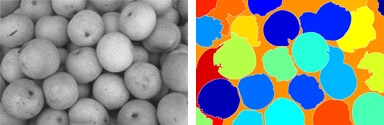
\includegraphics[width=0.8\textwidth]{figures/segmentation}
  \caption{Image Segmentation Example.}
  \label{fig:segmentation}
\end{figure}

\subsection{Region Growing}

Region growing is a simple region-based image segmentation method. It is also classified as a pixel-based image segmentation method since it involves the selection of initial seed points.

The main goal of segmentation is to partition an image into regions. Some segmentation methods such as thresholding achieve this goal by looking for the boundaries between regions based on discontinuities in grayscale or color properties. Region-based segmentation is a technique for determining the region directly. The basic formulation is:

\begin{enumerate}
\item Segmentation must be complete; that is, every pixel must be in a region.
\item Points in a region must be connected in some predefined sense.
\item Different regions must be disjoint.
\item All pixels in a common region must satisfy some common property.
\item If two regions are adjacent, they must be different in that predicate property.
\end{enumerate}

Seed points are selected to satisfy the requirements of the goal.

\section{Contour Detection}
Contours can be explained simply as a curve joining all the continuous points (along the boundary), having same color
or intensity. The contours are a useful tool for shape analysis and object detection and recognition.

Contours are the boundaries of a shape with same intensity. It stores the (x,y) coordinates of the boundary of a shape. But does it store all the coordinates ? That is specified by this contour approximation method. One such method, The Ramer–Douglas–Peucker algorithm, also known as the Douglas–Peucker algorithm and iterative end-point fit algorithm, takes a curve composed of line segments and finds a similar curve with fewer points.

``\Cref{fig:conapp} shows the Contour Approximation Procedure''.

\begin{figure}[h]
  \centering
  
\includegraphics[width=0.8\textwidth]{figures/conapp.png}
  \caption{Contour Approximation}
  \label{fig:conapp}
\end{figure}

\section{Template Matching}
Template Matching is a method for searching and finding the location of a template image in a larger image. Simply slides the template image over the input image (as in 2D convolution) and compares the template and patch of input image under the template image.

\section{Conclusion}
We need these terminologies described above in our thesis. Image conversion transforms scanned colored image to greyscale. Smoothing eliminates unacceptable noise points in the scanned image. Morphological operations further clear out noise points and join adjacent broken curved segments. Contour detection detects majority of the plot contours and objects. Template matching segments out the numbered pixels and eliminates them from the original image. Region growing forms a connected whole Plot raster image.

\endinput





% Another chapter
\chapter{Literature Review}\label{review}


\section{Introduction}
We need a lot more things to do for reconstructing a scene. Object needs to be recognized. Then need some way to track the movement of the object. And if some of the scenes are missing, then we need to construct that missing scenes. For that, we need to know the velocity, path and nature of the movement of that object to predict the future movement and construct that missing scenes.

In this chapter we will discuss various ground-level researches on \textbf{Image Processing} that will be very useful in our research. 


\subsection{This is a Subsection}
And some more.
\subsubsection{This is a Subsubsection}
Yet some more.

\section{And Another Section}




\endinput


% Chapter showing example of index creation

\usetikzlibrary{shapes,arrows}
\pagestyle{empty}

\chapter{Research Plan} \label{plan}

\section{Introduction}

The solutions discussed so far all have one thing in common. They provide very specific and satisfactorily accurate partial solution to the overarching process. But the complete automated feature extraction and analysis is not yet available. This work deals with a very specific standard of map where accuracy of both shape and scale are of paramount importance. All process should be completely automated for maximum efficiency. Moreover, none of these previous works deal with specific plot segmentation over a large constellation of closely arranged contours.

In this chapter we will describe problem formulation, our work plan, what we have already done and what have to be done in future. 

\section{Overview of the Problem}

A scanned paper Mouza map is taken as any available image format, such as : .png, .jpg, .bmp etc. Initially the scanned image will contain various distortions. But, after processing, the plot lines or remaining segments must form a single connected component ${C}$. Suppose after the contour analysis and template matching processes, the number of extracted number groupings are ${N}$. The image should be processed in such a way that the number of extracted plots ${n}$ match exactly with ${N}$. For that, some of the numbers that lie outside the connected component ${C}$ , equals ${r}$ must be subtracted from original numbered groups ${N}$. Transformations must be applied to obtain plot contours,
\begin{equation}
n=N-r, where r=C'
\end{equation}


\section{Work Plan}\label{todo}

We have divided our work to several steps. They are described below : 

\begin{enumerate}
    \item Removing background noise\ref{noise}
    \item Connecting broken contours\ref{closing}
    \item Contour size analysis\ref{segcon}
    \item Number detection\ref{template}
    \item Number segmentation\ref{remove}
    \item Plot contour extraction\ref{plot}
    \item Combining all the extracted subplots to make the whole mouza map\ref{merge}
\end{enumerate}


\section{Works Done So Far}

The steps \ref{noise}, \ref{segcon}, \ref{remove} and \ref{plot} described in section \ref{todo} are completed. They will be described elaborately in the following subsections.

\subsection{Noise Reduction}
Gaussian and Median filters are applied in succession. This reduces the amount of background noise. There are several specific kinds of noise prevalent in a scanned mouza map. They are mentioned below:
\begin{enumerate}
    \item Detecting moving objects in each frame
    \item Associating the detection corresponding to the same object over time
\end{enumerate}

The detection of moving objects uses a background subtraction algorithm based on Gaussian mixture models.~\cite{DBLP:conf/cvpr/StaufferG99} Morphological operations are applied to the resulting foreground mask to eliminate noise. Finally, blob analysis detects groups of connected pixels, which are likely to correspond to moving objects.

The association of detection to the same object is based solely on motion. The motion of each track is estimated by a Kalman filter. The filter is used to predict the track's location in each frame, and determine the likelihood of each detection being assigned to each track.

Track maintenance becomes an important aspect of this procedure. In any given frame, some detections may be assigned to tracks, while other detections and tracks may remain unassigned. The assigned tracks are updated using the corresponding detections. The unassigned tracks are marked invisible. An unassigned detection begins a new track.

Each track keeps count of the number of consecutive frames, where it remained unassigned. If the count exceeds a specified threshold, the example assumes that the object left the field of view and it deletes the track.

``\Cref{fig:moving} is the flowchart of tracking moving objects in a video frame.''



A short description of the total procedure is given below :

\begin{figure}[H]
  \centering
  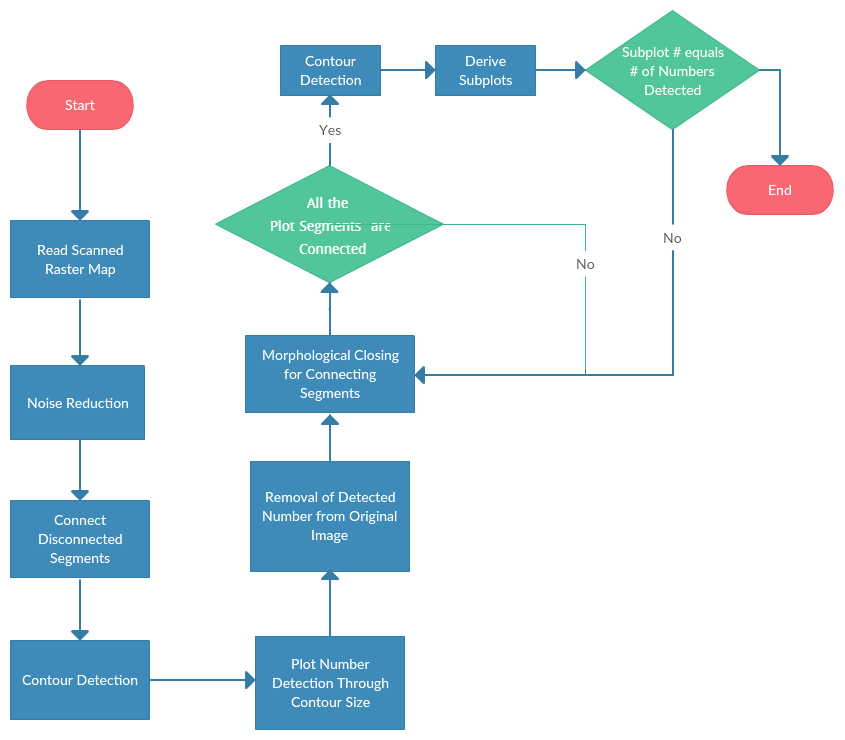
\includegraphics[width=0.9\textwidth]{figures/raster}
  \caption{Flowchart}
  \label{fig:raster}
\end{figure} 

\begin{enumerate}

    \item \textbf{Create System Object} : This is used for reading the video frames, detecting foreground objects, and displaying results. 
    
    \item \textbf{Initialize Tracks} : This creates an array of tracks, where each track is a structure representing a moving object in the video. The purpose of the structure is to maintain the state of a tracked object. The state consists of information used for detection to track assignment, track termination, and display. 
    
    \item \textbf{Read Frame} : This reads the next video frame from the video file. 
    
    \item \textbf{ Detect Objects} : The function returns the centroids and the bounding boxes of the detected objects. It also returns the binary mask, which has the same size as the input frame. Pixels with a value of 1 correspond to the foreground, and pixels with a value of 0 correspond to the background. The function performs motion segmentation using the foreground detector.~\cite{DBLP:conf/cvpr/StaufferG99} It then performs morphological operations on the resulting binary mask to remove noisy pixels and to fill the holes in the remaining blobs.
    
    \item \textbf{Predict New Locations of Existing Tracks}: This uses the Kalman filter to predict the centroid of each track in the current frame, and update its bounding box accordingly.
    
    \item \textbf{Assign Detections to Tracks} : This assigns object detections in the current frame to existing tracks is done by minimizing cost. ~\cite{Miller97optimizingmurty's,doi:10.1137/0105003}
    
    \item \textbf{Update Assigned Tracks} : The procedure updates each assigned track with the corresponding detection.
    
    \item \textbf{Update Unassigned Tracks} : This marks each unassigned track as invisible, and increases its age by 1.
    
    \item \textbf{Delete Lost Tracks} : This deletes tracks that have been invisible for too many consecutive frames. It also deletes recently created tracks that have been invisible for too many frames overall.
    
    \item \textbf{Create New Tracks} : This creates new tracks from unassigned detections assuming that any unassigned detection is a start of a new track.
    
    \item \textbf{Display Tracking Results} : This draws a bounding box and label ID for each track on the video frame and the foreground mask. It then displays the frame and the mask in their respective video players.
    
    \item \textbf{Are More Frames Available} : This checks if more video frame is available in the video clip. If it is yes, then it goes to read frame procedure and continues. If it is no then , stop the process. 
    
    
    
\end{enumerate}
   
\subsubsection{Experimental Results}
    
    We have done our experiment and simulation in MATLAB. In appendix \ref{ch:codes} at section \ref{trackcode} contains the code of tracking moving object in a video. ``Figure ~\ref{fig:car1}-~\ref{fig:man3} shows our experimental result of tracking moving objects with a boundary box in a video frame.''.

\begin{figure}[H]
  \centering
  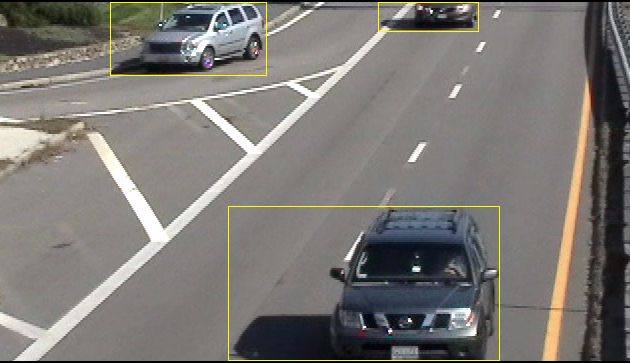
\includegraphics[width=0.9\textwidth]{figures/car1}
  \caption{Tracking Moving Objects Result.}
  \label{fig:car1}
\end{figure} 

\begin{figure}[H]
  \centering
  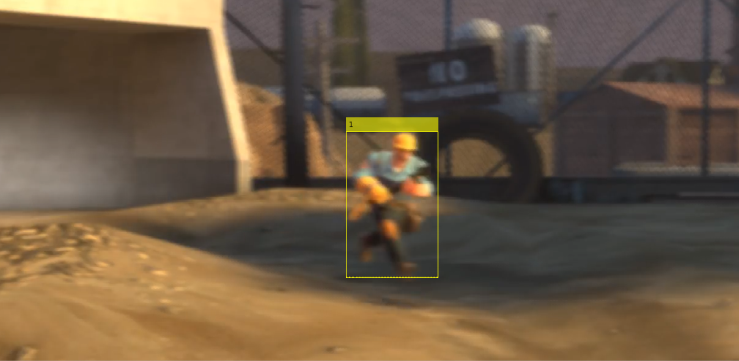
\includegraphics[width=0.9\textwidth]{figures/man1}
  \caption{Tracking Moving Objects Result.}
  \label{fig:man1}
\end{figure} 

\begin{figure}[H]
  \centering
  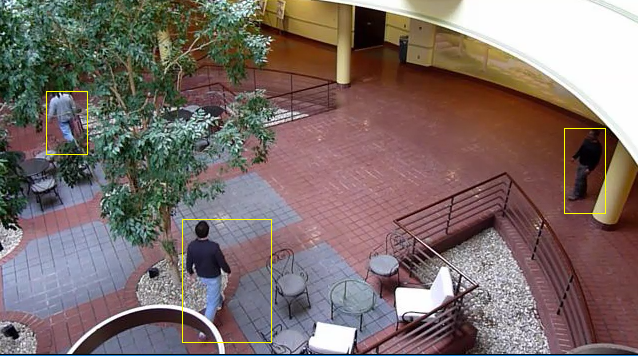
\includegraphics[width=0.9\textwidth]{figures/man3}
  \caption{Tracking Moving Objects Result.}
  \label{fig:man3}
\end{figure} 
    
Our experiment which is done in MATLAB shows good result of tracking moving objects with a boundary box in video frames.

\subsection{Tracking Velocity of Each Moving Object}\label{velocity}

After tracking moving objects, we have tracked velocity of each object . We've a boundary box associated with each object which have a centroid. In every frame, we have calculated the displacement of the centroid from the previous frame of the object. This value is velocity in  pixel per frame for that object. Multiplying it with frame rate, we got the instantaneous velocity for that frame for the object. After all the frame is explored, we divide the total displacement of that object in the video by the numbers of time the objects have appeared in all the video frames. This is the average velocity of the object in that video. The average velocity is needed when we want to predict an object's future movement. If frame rate r, total displacement in the video of a object $t_d$, number of the frames the object appears in the video n then , 
\newline
\newline
\centerline{displacement in X axis in pixel, x = centroidX - centroidX of previous frame}
\centerline{displacement in Y axis in pixel, y = centroidY - centroidY of previous frame}
\centerline{displacement in a frame in pixel, d = $\sqrt{x^2 + y^2}$}
\centerline{instantaneous velocity in pixel per second, v = d $\times r$}
\centerline{
total average velocity in the video, $v_{avg}$ = $\frac {t_d}{n}$
}

\subsubsection{Experimental Results}
    
In appendix \ref{ch:codes} at section \ref{trackcode} contains the code of tracking moving object with object id and velocity in a video.``Figure ~\ref{fig:car1v}-~\ref{fig:man3v} shows our experimental result of tracking moving objects with a boundary box in a video frame with object id and instantaneous velocity in pixel per second unit.''.

\begin{figure}[H]
  \centering
  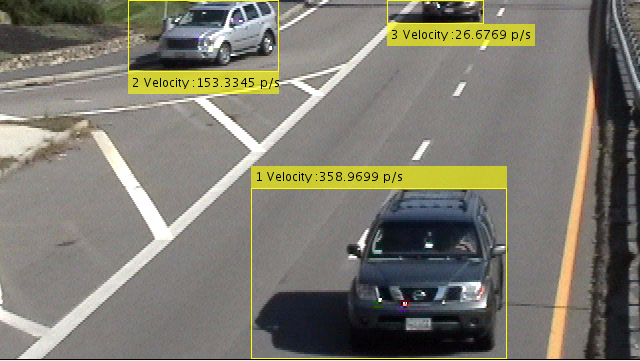
\includegraphics[width=0.9\textwidth]{figures/car1v}
  \caption{Tracking Moving Objects with Velocity in Pixel Per Second.}
  \label{fig:car1v}
\end{figure} 

\begin{figure}[H]
  \centering
  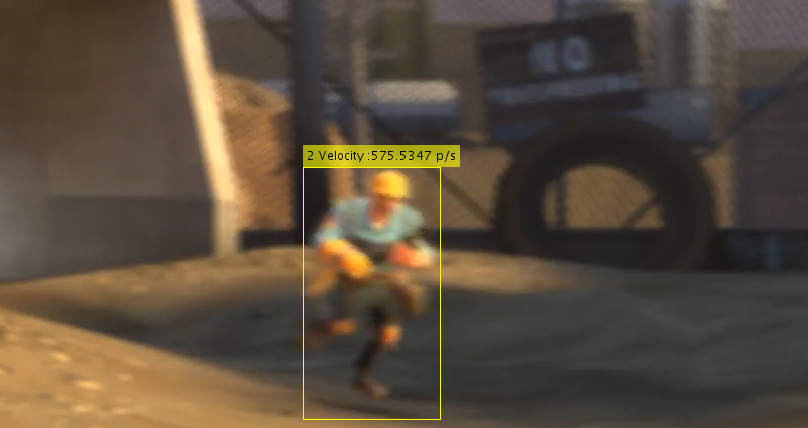
\includegraphics[width=0.9\textwidth]{figures/man1v}
  \caption{Tracking Moving Objects with Velocity in Pixel Per Second.}
  \label{fig:man1v}
\end{figure} 

\begin{figure}[H]
  \centering
  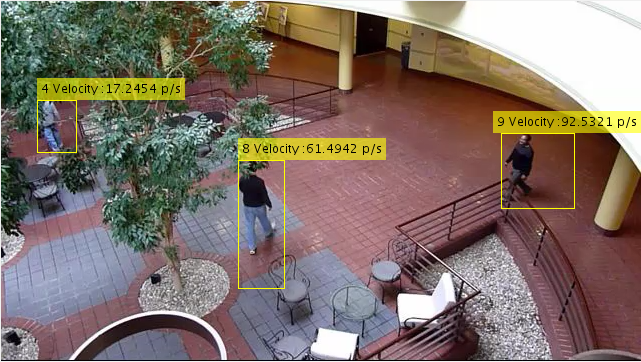
\includegraphics[width=0.9\textwidth]{figures/man3v}
  \caption{Tracking Moving Objects with Velocity in Pixel Per Second.}
  \label{fig:man3v}
\end{figure} 

\subsection{Determining Approximate Time through Prediction}

We need to predict how much time is needed by an object to pass an area where a camera is not available or the camera of the area is damaged. We can predict the time by its previous or future camera's average velocity. We've already got the average velocity described in section \ref{velocity}. Now we need a background image where a camera is not available or the camera is damaged. We also have to specify the path where the object might have passed. If we divide the total distance of the specified path by the average previous or future velocity, we will get an approximate time to pass the path for that object. If total distance is d and average velocity is $v_avg$ then,
\newline
\newline
\centerline{total approximate time, $t$ = $\frac{d}{v_{avg}}$}

\subsubsection{Experimental Results}
In appendix \ref{ch:codes} at section \ref{prediction} contains the code of determining approximate time given the object average velocity and the specified path in the background image of the area where there is no camera or the camera is damaged. ``\Cref{fig:background} shows a background image with specified path where camera not available.''.

\begin{figure}[H]
  \centering
  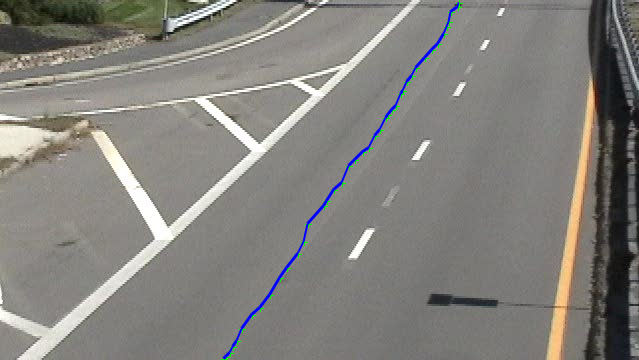
\includegraphics[width=0.9\textwidth]{figures/background}
  \caption{Background Image with Specified Path Where Camera Not Available.}
  \label{fig:background}
\end{figure} 

\endinput
 

% Bangla example, uncomment if you need this
% \chapter{Example of Bangla}

\section{Long Text in English}

This text is in English.

\bengalitext{আর এটা বাংলায় লেখা।}

Lorem ipsum dolor sit amet, consectetur adipiscing elit. Cras et
ultricies massa. Nulla a sapien lobortis, dignissim nibh in, aliquet
mauris. Integer at dictum metus. Quisque in tortor congue ipsum
ultricies tristique. Maecenas ut tortor dapibus, sagittis enim at,
tincidunt massa. Ut sollicitudin sagittis ipsum, ac tincidunt quam
gravida ac. Nullam quis faucibus purus. Aliquam vel pretium
turpis. Aliquam a quam non ex interdum sagittis id vitae quam. Nullam
sodales ligula malesuada maximus consequat. Proin a justo eget lacus
vulputate maximus luctus vitae enim. Aliquam libero turpis, pharetra a
tincidunt ac, pulvinar sit amet urna. Pellentesque eget rutrum diam,
in faucibus sapien. Aenean sit amet est felis. Aliquam dolor eros,
porttitor quis volutpat eget, posuere a ligula. Proin id velit ac
lorem finibus pellentesque.

\section{Long Text in Bangla}

\begin{bengali}
  মধ্যাহ্ন বিরতির পর রানের চাকা বেশ দ্রুতই ঘোরাচ্ছিলেন মুরালি বিজয় আর
  চেতেশ্বর পূজারা। ১৭৮ রানের জুটি গড়েছিলেন তাঁরা। অবশেষে মেহেদী হাসান
  মিরাজের বলে স্বস্তি ফিরেছে বাংলাদেশ-শিবিরে। তাঁর বলে মুশফিকুর রহিমকে ক্যাচ
  দিয়েছেন চেতেশ্বর পূজারা। আউট হওয়ার আগে করেছেন ৮৩ রান। অপর প্রান্তে মুরালি
  বিজয় অপরাজিত ৯৩ রানে। এ প্রতিবেদন লেখার সময় ভারতের সংগ্রহ ২ উইকেটে
  ২০১। উইকেটে এসেছেন বিরাট কোহলি।

  বিজয়-পূজারা জুটি বেশ আগেই শেষ করে দেওয়ার সুযোগ এসেছিল বাংলাদেশের সামনে।
  বিজয়কে রান আউট করার সুযোগ পেয়েও তা কাজে লাগাতে পারেননি মিরাজ।

  তাঁর করা ১৯তম ওভারের তৃতীয় বলটি স্কয়ার লেগের দিকে ঘুরিয়েছিলেন মুরালি
  বিজয়। স্কয়ার লেগে ডাইভ দিয়ে রান বাঁচান কামরুল ইসলাম। কিন্তু নন স্ট্রাইকিং
  প্রান্তের চেতেশ্বর পূজারা রানটি পুরো করার জন্য দৌড়ালে প্রথমে বিজয় সাড়া দিতে
  চাননি। দুই ব্যাটসম্যানই ছিলেন একই প্রান্তে। পরে বিজয় নন স্ট্রাইকিং প্রান্তের
  দিকে দৌড় শুরু করেন। কামরুলের থ্রো বোলার মিরাজ ঠিকমতো ধরতে না পারায়
  নিশ্চিত রান আউটের হাত থেকে বেঁচে যান বিজয়।
\end{bengali}

% Chapter with math in ttile
\chapter{$k$-safe Labeling of Petersen Graph}\label{safeklabelingpetersen}

In 1898, Petersen produced a trivalent graph with no leaves, now
called the Petersen graph~\cite{holton1993petersen}.  In this chapter
we study $k$-safe labeling for the Petersen graph. We also give upper
bound for the span of the Petersen graph. We provide necessary proof
for the upper bound.

\endinput



% Bibliographies and appendices
% You do not need to change anything in this file. If you want to
% change the reference style, comment/uncomment the \bibliographystyle
% lines

\clearpage
\renewcommand\bibname{References}
\addcontentsline{toc}{chapter}{References}

% Comment/uncomment as suits you
\bibliographystyle{ieeetr} %% IEEE transaction style
% \bibliographystyle{acm} %% ACM style
% \bibliographystyle{alpha}
\bibliography{buetcseugthesis}

\endinput


% Index, comment this out if you do not want to create an index
\printindex

\appendix
% Algorithms
\chapter{Algorithms}\label{ch:algorithms}

\section{Sample Algorithm}
In Algorithm~\ref{alg1} we show how to calcute $y=x^n$.

\begin{algorithm}
  \caption{Calculate $y = x^n$}
  \label{alg1}
  \begin{algorithmic}
    \input{algorithms/yxn.alg}
  \end{algorithmic}
\end{algorithm}

\endinput


% Codes
% Code settings
\lstset{language=Matlab,%
    %basicstyle=\color{red},
    breaklines=true,%
    morekeywords={matlab2tikz},
    keywordstyle=\color{blue},%
    morekeywords=[2]{1}, keywordstyle=[2]{\color{black}},
    identifierstyle=\color{black},%
    stringstyle=\color{mylilas},
    commentstyle=\color{mygreen},%
    showstringspaces=false,%without this there will be a symbol in the places where there is a space
    numbers=left,%
    numberstyle={\tiny \color{black}},% size of the numbers
    numbersep=9pt, % this defines how far the numbers are from the text
    emph=[1]{for,end,break},emphstyle=[1]\color{red}, %some words to emphasise
    %emph=[2]{word1,word2}, emphstyle=[2]{style},    
}

\chapter{Codes}\label{ch:codes}

\section{Tracking Moving Objects and Velocity of Each Object in a Video} \label{trackcode}

\lstinputlisting{codes/ok.m}

\section{Predicting Approximate Time}\label{prediction}
\lstinputlisting{codes/myplotter.m}

\endinput


\end{document}
